
\section{Organisation und Aufbau}


Das Projekt ist entlang der unterschiedlichen Aufgaben modular organisiert. Unter dem Dach der Anwendung finden sich vier unterschiedliche Sparten, die gemeinsam für das Ausführen des Programms verantwortlich sind: Planknoten und Äuqivalenzklassen, Regeln und Regelsets, Executoren und Services. Die genaue Zuordnung zu den jeweiligen Bereichen ist in Abb. \ref{ProjectOrga} nachvollziehbar.


\begin{figure}[h]
  \centering
  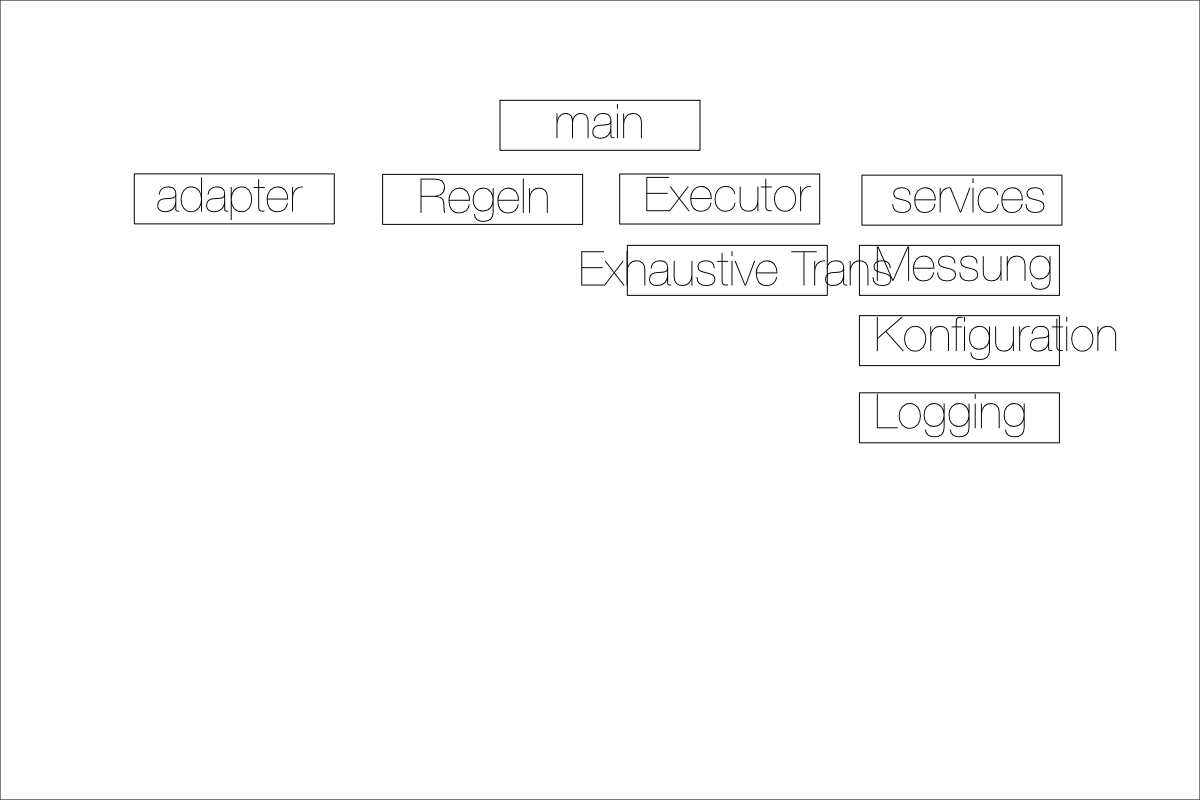
\includegraphics[width=\textwidth]{04_Implementierung/Matrix.png}
  \caption{Projektorganisation}
  \label{ProjectOrga}
\end{figure}

Bei der Ausführung eines Tests  müssen alle Bereiche zusammenarbeiten. Der Service-Bereich und insbesondere das Konfigurationsmodul sind für die konkrete Zusammenstellung der für den Test notwendigen Komponenten verantwortlich. Er entscheidet, welche Regeln zum Einsatz kommen, welcher Exector gewählt wird, welche konkreten Pläne getestet und mit Hilfe welcher Adapter die Daten ein-  bzw. ausgegeben werden. Um zu verstehen, welche Möglichkeiten das implementierte System bietet, sind die einzelnen Komponenten im Folgenden im Detail beschrieben.


\section{Services}

Da für die Ausführung des Programms unterschiedliche Dienstleistungen benötigt werden, die auch in anderen Kontexten relevant sein können, falls das Projekt diese Funktionen im Bereich Services zusammen. Teil des Bereichs ist der Konfigurator, der die Konfiguration der Tests übernimmt, die Zeitmessung und Das Logging von Informationen.

Nicht alle Komponenten wurden selbst entwickelt, beispielsweise wurde beim Logging auf die existierende Library easylogging++ gesetzt.

\subsection{Konfiguration}


\begin{figure}[ht]
  \centering
  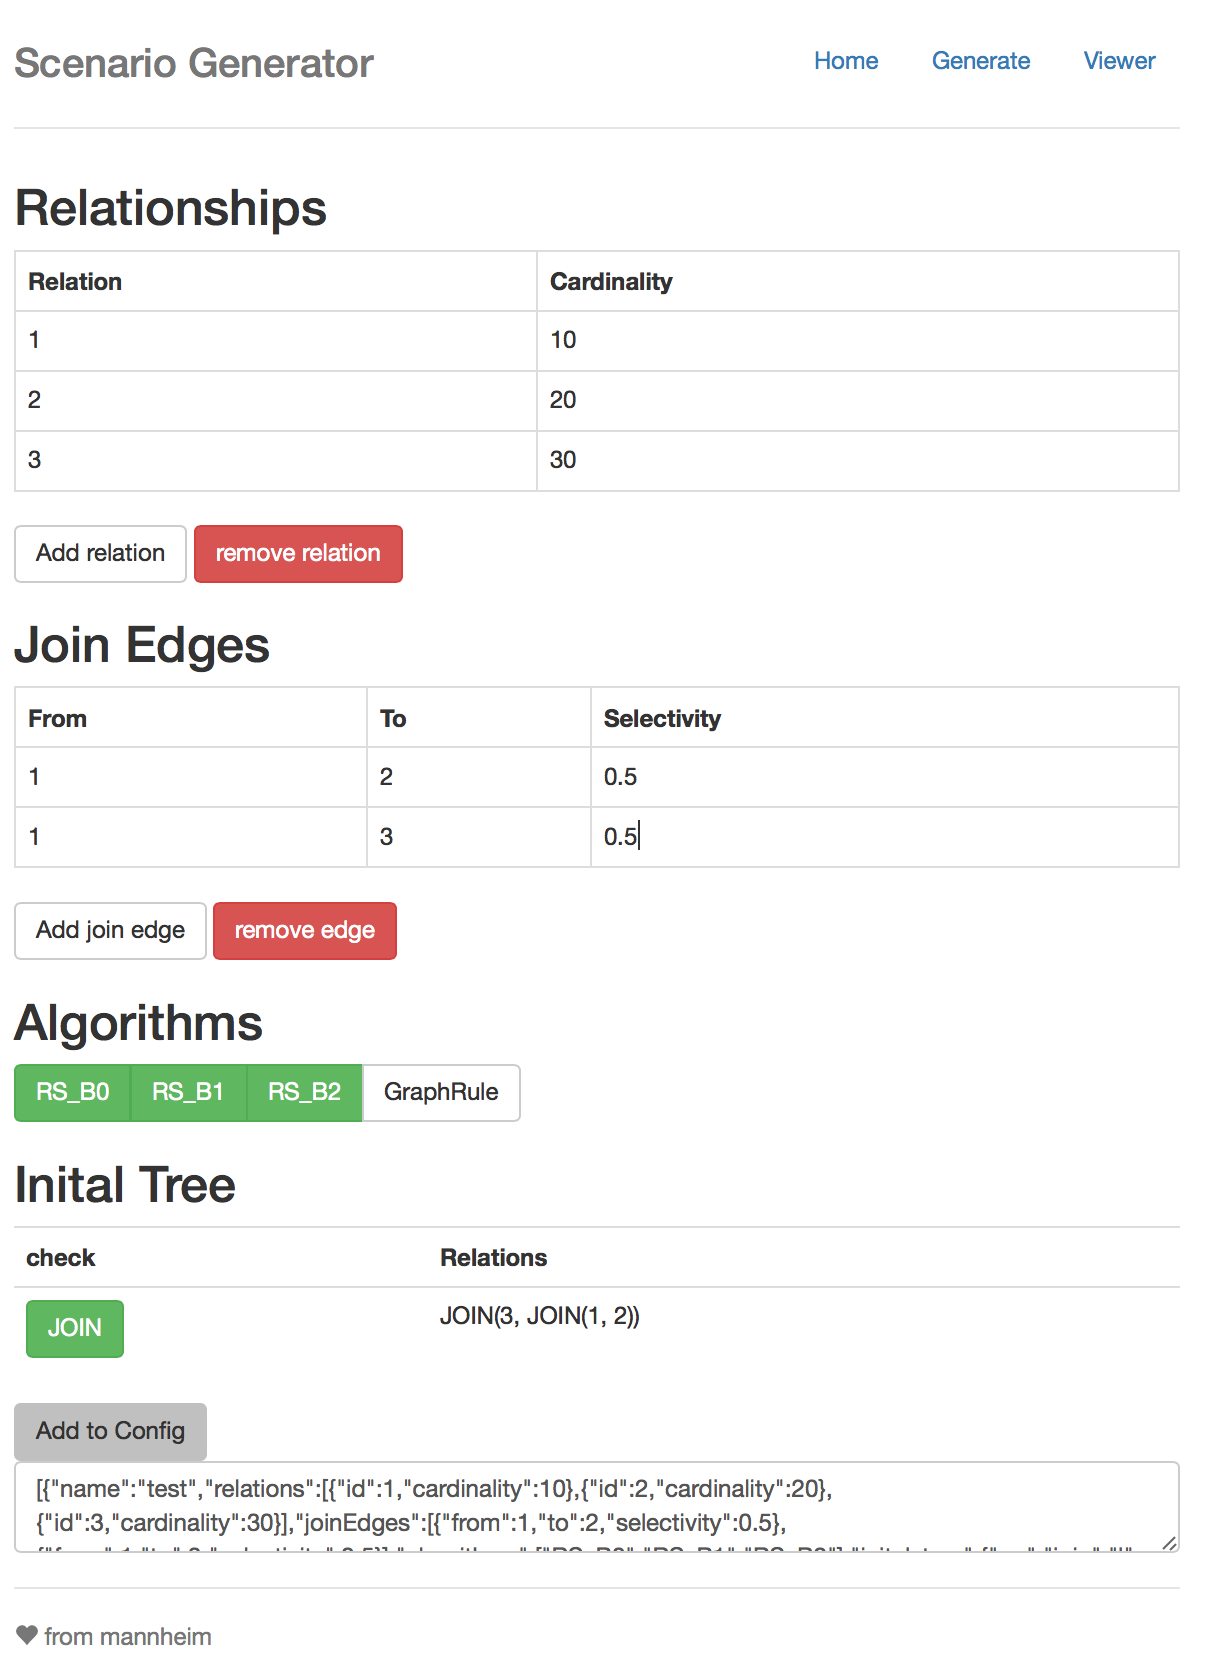
\includegraphics[width=0.5\textwidth]{04_Implementierung/ScenarioGenerator.png}
  \caption{Konfigurationstool: Scenario-Generator}
  \label{ScenarioGenerator}
\end{figure}

Das Konfigurationsmodul besteht aus zwei Komponenten. Auf der einen Seite eine Javascript-HTML Anwendung zur Generierung von Test-Szenarien (vgl. Abb. \ref{ScenarioGenerator}). Mit Hilfe dieser Anwendung können Konfigurationsfiles für den späteren Test erstellt werden. Dieses Konfigurationssystem, das in  zu sehen ist, bietet dem Nutzer die Möglichkeit Relationen mit Kardinalitäten zu erzeugen, Selektivitäten festzulegen und schlussendlich einen initalen Query Tree zu erzeugen. Ebenfalls ist es möglich die verschiedenen Regelsets, die geprüft werden sollen, festzulegen.
Das Ergebnis dieses Moduls ist eine Konfigurationsdatei im JSON Format. Das Tool unterstützt die Erzeugung mehrerer Secenarios in einem Konfigurationsfile. So können mehrere Scenarios in einem Test-Run durchgespielt werden.

Die eigentliche Konfiguration findet in C++ statt. Mit der Library json11 \cite{json11} wird das Konfigurationsfile gelesen. Für jedes Szenario und jedes Regelset wird ein initaler Baum aus Äquivalenzklassen und Planknoten mit einem JSON-Adapter gebildet. Der Exekutor wird gewählt und mit einem Regelset initialisiert. Der initiale Baum wird dem Exekutor übergeben. Nachdem die Regeln angewendet wurden, startet der Konfigurator die Kostenschätzung. Nachdem alle Szenarios abgearbeitet sind, ist das Programm beendet.

\subsection{Zeitmessung}
Wie bereits in Abb. \ref{Ablauf} dargestellt wird die Zeitmessung nach der Konfiguration gestartet. Sobald alle Pläne expandiert sind und die Kosten berechnet sind wird die Messung beendet. Um eine möglichst genaue Messung durchführen zu können, wurde die Uhr \texttt{std::chrono::steady\_clock} verwendet. Diese Uhr ist Teil von C++11. Wie in der Dokumentation \cite{cppreference_2015_clock} beschrieben handelt es sich bei der Uhr um eine monotone Uhr. Die Uhr kann nicht rückwärts laufen, solange die physische Zeit fortfährt. Die Uhr selbst mit der Wall\-Clock\-Time verbunden und ist das passende Werkzeug zur Messung von Intervallen. 

Die Dauer zwischen Start der Expansion und dem Ende der Kostenberechnung wird in Nanosekunden gemessen, um ein möglichst akkurates Ergebnis zu erhalten. Die gemessenen Ergebnisse werden sowohl als Debug-Log in der Konsole ausgegeben, aber auch in einem Log File gespeichert.



\subsection{Logging und Debugging}

Auch zum Debugging wurde eine externe Bibliothek eingesetzt: EasyLogging++ \cite{easylogging}, ein einfach zu bedienendes jedoch hochgradig konfigurierbares Logging Instrument. Gerade die Leichtgewichtigkeit - das Tool besteht nur aus einer Headerklasse -, die einfache Bedienung und Geschwindigkeit gabem den Ausschlag zur Nutzung der Library. Mit Hilfe dieser Library werden debugging Informationen geschrieben, aber auch Zeitmessungen gespeichert, pläne ausgegeben und sonstige Debugging Nachrichten ausgegeben. Insbesondere ist die Unterscheidung zwischen unterschiedlichen Debug\-Leveln wichtig. Auf mehreren Ebenen (INFO, WARNING, DEBUG, etc.) können Informationen ausgegeen werden. Je nachdem welches Level angesprochen ist, werden nur Informationen über dieses ausgegeben. 


\section{Adapter}

Die Implementierung bietet mehrere Adapter, die zur Umwandlung von externen Formaten in eine interne Repräsentationsform oder von einer internen Repräsentationsform in ein externes Format genutzt werden können. Sie bieten die Möglichkeit andere Systeme an das bestehende System anzudocken und sorgen so für den notwendigen Anschluss und die Erweiterbarkeit durch Dritte.

Insgesamt werden drei Adapter mitgeliefert. (1) JSON\-Adapter, (2) String\-Adapter, (3) DOT\-Adapter.

Der Json-Adaper erlaubt des Daten im JSON Format zu importieren und wird beim einlesen des initalen Plans genutzt. Er wandelt auf Basis des Konfigurationsfiles JSON in Planknoten und Äquivalenzklassen um, die dann weiterverarbeitet werden können. Ebenfalls ist es möglich Pläne in JSON auszugeben. Zu diesem Zweck implementiert der Parser auch eine \texttt{dump} Methode.

Neben dem JSON\-Adapter wird auch ein String Adapter verwendet. Er ist für die Ausgabe von Plänen als String verantwortlich. Im Gegensatz zu einem JSON\-Adapter ist die Eingabe von Plänen mit Hilfe dieses Moduls nicht möglich. Auch der DOT\-Adapter erlaubt nur die Ausgabe von Plänen im DOT\-Format. Das zur Generierung von graphischen Ausgaben verwendet werden kann.

Eine weitere Aufgabe eines solchen Adapters kann auch die Übersetzungen von Relationsnamen in Bitvektoren sein. Da das vorliegende System, wie in \ref{sec:Bitvector} beschrieben, Relationen als Bitvektoren abbildet, mag es nützlich sein, Relationsnamen in Bitvektoren zu übersetzen. Für diese Übersetzung sind auch Adapter vorgesehen, die zusätzlich implementiert werden können.




\section{Regeln und Regelsets}

\subsection{Regeln}

\subsection{Regelsets}


\section{Relationen, Planknoten und Äquivalenzklassen}

\subsection{Verwaltung von Relationen}
\label{sec:Bitvector}


\begin{figure}[ht]
  \centering
  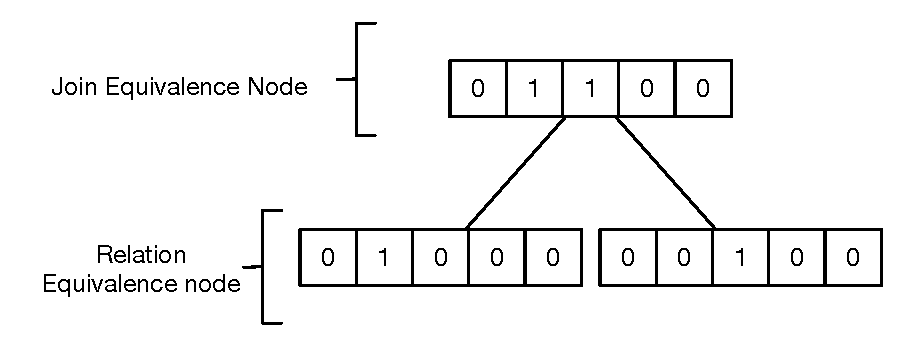
\includegraphics{04_Implementierung/Bitvector.pdf}
  \caption{Bitvekotren als Repräsentation von Relationen oder Joins}
  \label{Bitvektor}
\end{figure}

Die einzelnen Relationen werden mit Hilfe von Bitvektoren repräsentiert. Ein Bitvektor sind mehrere Bits, die entweder $TRUE$ also $1$ oder $FALSE$ also $0$ sein können. Ist das n-te Bit eines Bitvektors gesetzt, so repräsentiert dieses Bit die n-te Relation. Beispielsweise bezeichnet der Bitvektor $010000000$ die Relation mit dem Namen $1$. Mit Hilfe des Bitvektors können auch mehrere Relationen gespeichert werden $01010000000$ bezeichnet folglich die Relation mit dem Name $1$ und die Relation mit dem Namen $3$. Für die durchgeführten Berechnungen ist es nicht notwendig, dass eine Relation mit ihrem tatsächlichen Namen bekannt ist. Es reicht eine Bezeichnung mit Hilfe von Nummern aus.

Vorteil für die Verwendung von Bitvektoren ist, dass einfach Mengenoperationen durchgeführt werden können. So kann einfach geprüft werden, ob Äquivalenzklassen gemeinsame JOIN Kanten besitzen oder neue Relationen einer Äquivalenzklasse hinzugefügt werden. (vgl. Abb. \ref{Bitvector}) Dies ist besonders effizient, da nur Bits und keine komplexen Objekte wie Strings verarbeitet werden müssen.


Für externe Systeme kann es daher notwendig sein, dass Relationsnamen mit Hilfe eines Adapters übersetzt werden. Die genau Funktionsweise eines solchen Adapters wird in diesem Kapitel genauer beschrieben.




\subsection{Planknoten und Äquivalenzklassen}





\begin{figure}[h]
  \centering
  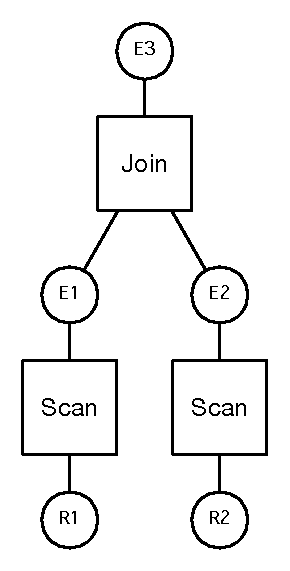
\includegraphics{04_Implementierung/JoinScan.pdf}
  \caption{Planknoten und Äquivalenzklassen}
  \label{PlanAequi}
\end{figure}

Zu  Beginn steht die Struktur in der Pläne gespeichert werden. Diese Struktur wird durch andere Komponenten bearbeitet und ausgewertet und stellt somit das Werkstück bei der Verarbeitung dar.

Ähnlich wie in anderen System kommen in der aktuellen Implementierung Äquivalenzklassen und Planknoten zum Einsatz. Äquivalenzklassen repräsentieren ein Set von unterschiedlichen, jedoch äquivalenten Planknoten. Mit Hilfe von Äquivalenzklassen und Planknoten kann die Information über alle möglichen Äquivalenten Pläne gespeichert werden. Sie können also den gesamten Search Space abbilden.
 Aufgabe eines Planknotens ist es einen Operator zu repräsentieren. Jeder Operator kann mehrere Parameter besitzen. Im konkreten Fall sind zwei Operatoren implementiert: JOINs und SCANs. Scans zeichnen sich dadurch aus, dass sie immer genau eine Relation lesen. Folglich haben Sie nur einen Parameter, um die Relation zu übergeben. Bei Joins gibt es immer genau zwei Parameter. Beide Parameter repräsentieren Datenströme, die mit Hilfe des Joins in einen gemeinsamen Datenstrom kombiniert werden.

Die kleinste im System mögliche Datenstruktur ist ein Scan. Er besteht aus einer Äquivalenzklasse, die die Relation repräsentiert. Auf sie wird ein Planknoten angewendet mit dem Operator SCAN. Dieser Planknoten ist selbst wieder Teil einer Äuqivalenzklasse. Eine solche Datenstruktur ist im linken Teil der Abbildung \ref{PlanAequi} zu finden.

Kombiniert man zwei dieser SCANs mit einem JOIN so erhält man die kleinste mögliche Struktur, die einen JOIN beinhaltet. Dies ist in Abb. \ref{PlanAequi} zu sehen. In diesem konkreten Fall ist noch keine Transformation auf den bestehenden Graphen angewendet worden. Es existieren also noch keine alternativen Planknoten. Eine solche Transformation könnte beispielsweise zur Folge habe, dass neben dem bisher bestehenden JOIN Knoten ein neuer JOIN Knoten erzeugt wird, der die beiden untergeordneten Relationen in umgekehrter Reihenfolge joint.


\subsection{Konkrete Implementierung}

Die konkrete Implementierung der Äquivalenzklasse sieht vor, wie in Abb. \ref{EquivalenceClassDiagram} zu erkennen, dass für jede Äquivalenzklasse die darin aggregierten Relationen sowie deren Nachbarn gespeichert werden. Ebenfalls wird der erste, letzte und kosteneffektivste Planknoten gespeichert. Außerdem kann festgehalten werden, ob eine Äquivalenzklasse bereits $explored$, also erforscht, ist. 






\subsection{Exektuoren}










\section{Regeln und Regelsets}


Eine entscheidende Komponente sind Regeln und Regelsets. Mehrere Regeln werden in einem Regelset zusammengefasst. Ein Regelset ist eine Instanz der abstrakten Klasse $RuleSet$, die die Methode $getRules()$ vorgibt, mit deren Hilfe ein Vektor von Regeln ausgegeben wird. Je nach Regelset können andere Regeln vorhanden sein.







\subsubsection{Organisation von Regeln}


\begin{figure}[h]
  \centering
  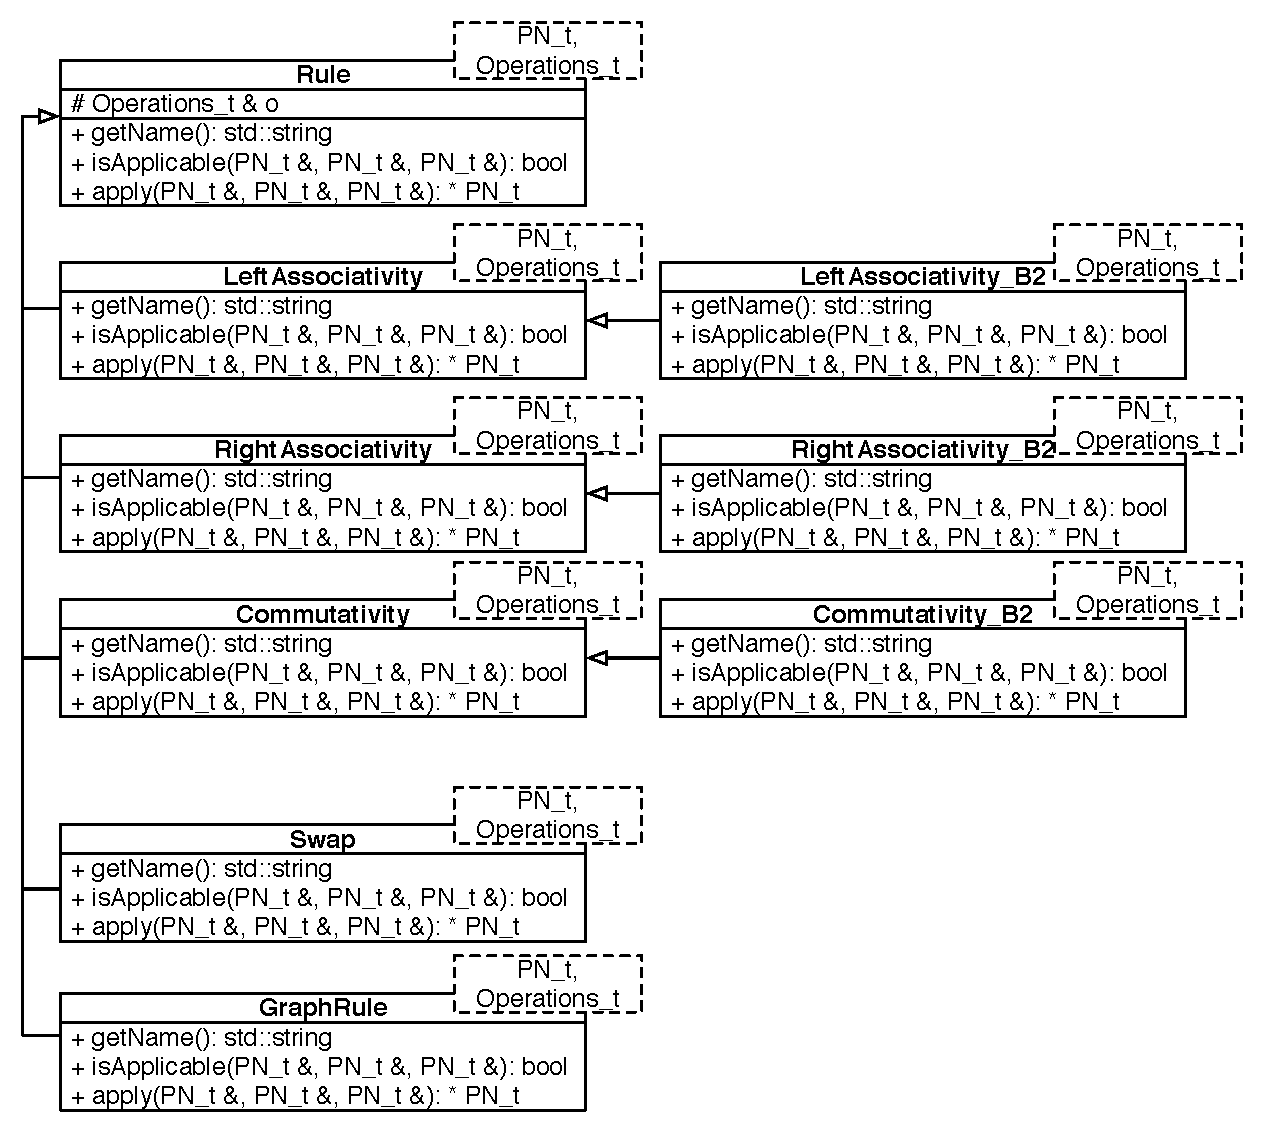
\includegraphics[width=\textwidth]{04_Implementierung/Rules.pdf}
  \caption{Regeln und Regelsets Klassendiagramm}
  \label{RuleClassDiagram}
\end{figure}


Auch bei den Regeln erben alle Regeln direkt oder - und das ist neu - indirekt von der Klasse $Rule$. Die Organisation der Klassen ist in Abb. \ref{RuleClassDiagram} dargestellt. Insgesamt wird zwischen den Regeln auf drei Ebenen unterschieden: 

$Commutativity$, $LeftAssociativity$ und $RighAssociativity$ bilden die erste Ebene der Regeln. Sie kommen in Verbindung mit den RuleSets $RS_0$ und $RS_1$ zum Einsatz.

Auf dem zweiten Level, diese Klassen sind mit dem Zusatz $B2$ gekennzeichnet, finden sich $Commutativity_B2$, $LeftAssociativity_B2$, $RighAssociativity_B2$ und $Exchange_B2$. Diese Regeln sind für das Regelset $RS_2$ notwendig und erlauben es andere Regeln zu deaktivieren. Da die Deaktivierung von Regeln eine Erweiterung darstellt, erben Kommutativität und Assoziativität von ihren Verwandten aus $RS_0$ bzw. $RS_1$. Da die Exchange Regel neu hinzukommt, erbt diese direkt von Rule.

Auf dem dritten Level findet sich die $GraphRule$. Sie ersetzt andere Regeln und ist im RuleSet $GraphRuleSet$ abgebildet.


Ähnlich wie bei Starburst bestehen Regel aus zwei Teilen. Auf der einen Seite wird geprüft, ob eine Regel zur Anwendung kommen kann. Dies geschieht mit der Methode $isApplicable$ auf der anderen Seite gibt es die Methode $apply$, die immer einen äquivalenten Planknoten zurückliefert. Mit Hilfe dieses Prinzips wurden alle Regeln implementiert. Das einheitliche Interface erlaubt es, dass Regeln in Regelsets gebündelt werden können.


\subsubsection{Erweiterbarkeit von Regeln}

Die Erweiterbarkeit ist auf mehreren Ebenen sichergestellt. Auf der einen Seite können neue Regeln erzeugt werden. Sobald diese die Form der abstrakten Klasse $Rule$ übernehmen, können sie in Regelsets zum Einsatz kommen. Ein Beispiel für eine solche Erweiterung ist die Regel $GraphRule$. Sie wurde später der entwickelten Lösung hinzugefügt. Das neue RuleSet $GraphRuleSet$ beinhaltet in diesem speziellen Fall nur eine Regel.

Eine weitere Möglichkeit zur Erweiterung wurde ebenfalls von $GraphRule$ genutzt. GraphRule gibt nicht nur einen einzelnen neuen Planknoten zurück, sondern übergibt gleich einen vollständig expandierten Baum. Auch diese Anforderung konnte ohne Veränderung des Interfaces umgesetzt werden. Da der Planknoten ein $next$ Attribut besitzt, das den vorhergehenden mit dem nächsten Knoten verbindet, können Ketten von neuen Knoten gebildet werden. Diese Ketten werden im Falle der $GraphRule$ zurückgegeben ohne dabei das Interface zu brechen.

Neben den vorgegebenen  Methoden können auch weitere Methoden für eine Regel implementiert werden. Dies ist beispielsweise bei $GraphRule$ notwendig gewesen. Hier ist es erforderlich, dass der Graph zuerst partitioniert wird, dann ConnectedComponents gefunden und schlussendlich ein Baum zurückgegeben wird. Auch dies ist innerhalb der Rules möglich.

Eine weitere Möglichkeit zur Erweiterung ist durch Templates gegeben. Template ist eine Funktion von C++ mit deren Hilfe Funktionen und Klassen mit generischen Typen arbeiten können. Dadurch ist es einer Funktion der einen Klasse möglich viele unterschiedliche Typen zu unterstützen ohne die Funktion oder die Klasse bearbeiten zu müssen. Im konkreten Fall der Regeln werden zwei dieser generischen Typen verwendet: $PlanNode$ und $Operations$. Es wird somit möglich die Klassen des Planknotens und die möglichen Operationen, die für diese Planknoten möglich sind zu ersetzen, ohne Funktionen und Klassen verändern zu können.

\subsubsection{Erweiterbarkeit von Regelsets}

Auch die Erweiterung von Regelsets ist möglich. Mit Hilfe neuer Regelsets, kann eine neue Reihenfolge bei der Ausführung definiert werden. Eine weitere Priorisierung von Regeln ist bisher nicht vorgesehen. Es ist jedoch möglich mit Hilfe der Methode $getRules()$, die für jedes Regelset implementiert ist, eine spezielle Priorisierung zu implementieren. 

Neben der Priorisierung sind auch neue Zusammenstellungen möglich. Beispielsweise ist der Unterschied zwischen $RS_0$ und $RS_1$ nur, dass eine Assoziativ-Regel weggelassen wurde. Ein Mix von alten und neuen Regeln ist möglich.

Wird ein neues Regelset erstellt, ist es nicht nur notwendig eine neue Regelset Klasse zu erstellen, sondern auch diese für das Ausführen im Executor anzumelden. Der Executor muss also ebenfalls angepasst werden.



\subsection{Ausführung von Regeln}

Das eigentliche Ausführen der Regeln wird durch einen XY durchgeführt. Im konkreten Fall kommt hier der Algorithmus ExhaustiveTransformation zum Einsatz. Der Algorithmus startet mit einer Äquivalenzklasse. Innerhalb dieser Äquivalenzklasse werden die Regeln, die durch ein Regelset vorgegeben sind auf einem PlanKnoten ausgeführt. Die Ausführung geschieht hierbei zuerst auf den Oberen Ebenen und setzt sich dann auf den Kindern eines Knoten fort. Somit können bei der Transformation eines gegebenen Baums alle Regeln auf andere Bäume angewendet werden.

Wichtig ist hierbei zu bemerken, dass dieser Algorithmus immer zuerst prüft, ob eine Regel auch tatsächlich für die Anwendung geeignet ist und dann erst der Algorithmus ausgeführt wird. Neben der eigentlichen Eignung wird auch geprüft, ob eine Äquivalenzklasse bereits vollständig expandiert wurde. Falls dies der Fall ist, wird von einer weiteren Anwendung von Regeln abgesehen. Diese Funktion kann insbesondere Vorteile bei der Implementierung von neuen Regelsets bieten. Nutzt ein gegebenes Regelset die Möglichkeit nicht nur einen neuen Planknoten zu generieren, sondern gleich mehrere Planknoten zu erstellen und auch in diesem Zusammenhang bereits mehrere Kinder-Knoten zu erstellen, kann die Reihenfolge der Expansion von Äuqivalenzklassen geändert werden. Die einzelnen Äquivalenzklassen, die bereits durch eine Regel expandiert wurden, werden als solche markiert und die bisher vorhandenen Regeln werden nicht mehr ausgeführt.


\section{Kostenschätzung und statistische Informationen}



Die Kostenschätzung zur Suche des optimalen Plans geschieht bei der vorliegenden Implementierung in einem eigenen Kostenschätzungsmodul.Teil des Kostenmoduls ist ein Katalog innerhalb dessen Informationen über Selektivität von JOINs und Kardinalitäten von Relationen gespeichert sind. Diese Informationen werden aus dem Katalog mit Hilfe des Kostenschätzers ausgelesen und die Kosten für einen Planknoten berechnet.

Die Berechnung der Kardinalität findet bottom up statt. Für jede Äquivalenzklasse wird die optimale Kardinalität berechnet und gespeichert. Der Planknoten mit dessen Hilfe diese optimale Kardinalität erreicht wird, wird als bester Planknoten markiert. Folgt man dem Pfad der besten Planknoten ergibt sich der kostenoptimale Baum an Planknoten. Die Berechnung sieht vor, dass immer die Selektivität eines Operators mit dem Produkt der Kardinalität der Eingabeparameter multipliziert wird. Beispielsweise wird auf der untersten Ebene - der Ebene der Scans - für eine gegebene Relation die Kardinalität mit der Selektivität von 1 multipliziert, da die gesamte Relation verarbeitet werden muss. Bei einem Join können komplexere Situationen auftreten. Zuerst wird das Produkt der Kardinalität der Eingabe Parameter berechnet. Diese kann dann mit der 
Selektivität multipliziert werden. Das Produkt der Kardinalitäten repräsentiert in diesem Falle die Kardinalität des möglichen Kreuzproduktes, das mit Hilfe von Selektoren eingeschränkt wird.



\subsection{Zusammenfassung}

Gerade im Bereich der Regeln ist klar zu erkennen, dass die SOLID Prinzipien eingehalten wurden. Hier ist jede Klasse nur für genau eine Aufgabe zuständig. Ein hohes Maß an Kohäsion konnte erreicht werden. Die Regelklassen  sind offen für Erweiterungen, jedoch geschlossen für Modifikationen. Dies wird insbesondere bei der Erweiterung mit Hilfe des Regelsets $GraphRuleSet$ deutlich. Auch das Liskov Substitutionsprinzip wurde eingehalten. Alle Klassen verhalten sich nach außen gleich und liefern dasselbe Ergebnis, einen Planknoten, zurück. 